%% This is file `elsarticle-template-1-num.tex',
%%
%% Copyright 2009 Elsevier Ltd
%%
%% This file is part of the 'Elsarticle Bundle'.
%% ---------------------------------------------
%%  
%% It may be distributed under the conditions of the LaTeX Project Public
%% License, either version 1.2 of this license or (at your option) any
%% later version.  The latest version of this license is in
%% http://www.latex-project.org/lppl.txt
%% and version 1.2 or later is part of all distributions of LaTeX
%% version 1999/12/01 or later.
%% 
%% Template article for Elsevier's document class `elsarticle'
%% with numbered style bibliographic references
%% 
%% $Id: elsarticle-template-1-num.tex 149 2009-10-08 05:01:15Z rishi $
%% $URL: http://lenova.river-valley.com/svn/elsbst/trunk/elsarticle-template-1-num.tex $
%% 
%%\documentclass[preprint,12pt]{elsarticle}

%% Use the option review to obtain double line spacing
%% \documentclass[preprint,review,12pt]{elsarticle}

%% Use the options 1p,twocolumn; 3p; 3p,twocolumn; 5p; or 5p,twocolumn
%% for a journal layout:
%% \documentclass[final,1p,times]{elsarticle}
%% \documentclass[final,1p,times,twocolumn]{elsarticle}
%% \documentclass[final,3p,times]{elsarticle}
\documentclass[preprint,3p,times,number]{elsarticle}
%% \documentclass[final,5p,times]{elsarticle}
%% \documentclass[final,5p,times,twocolumn]{elsarticle}

%% The graphicx package provides the includegraphics command.
\usepackage{graphicx}
%% The amssymb package provides various useful mathematical symbols
\usepackage{amssymb}
%% The amsthm package provides extended theorem environments
%% \usepackage{amsthm}
\usepackage[table,xcdraw]{xcolor}
%% The lineno packages adds line numbers. Start line numbering with
%% \begin{linenumbers}, end it with \end{linenumbers}. Or switch it on
%% for the whole article with \linenumbers after \end{frontmatter}.
\usepackage[utf8]{inputenc}
\usepackage{lineno}
\usepackage{csquotes}
\usepackage[all]{nowidow}
\usepackage{microtype}
\usepackage{tabularx}
\usepackage{booktabs}
\usepackage{wasysym}
\usepackage{calc}
\usepackage{tikz}
\usepackage{subcaption}
\usepackage{stfloats}
\usepackage{url}
\usepackage{todonotes}

%% natbib.sty is loaded by default. However, natbib options can be
%% provided with \biboptions{...} command. Following options are
%% valid:

%%   round  -  round parentheses are used (default)
%%   square -  square brackets are used   [option]
%%   curly  -  curly braces are used      {option}
%%   angle  -  angle brackets are used    <option>
%%   semicolon  -  multiple citations separated by semi-colon
%%   colon  - same as semicolon, an earlier confusion
%%   comma  -  separated by comma
%%   numbers-  selects numerical citations
%%   super  -  numerical citations as superscripts
%%   sort   -  sorts multiple citations according to order in ref. list
%%   sort&compress   -  like sort, but also compresses numerical citations
%%   compress - compresses without sorting
%%
%% \biboptions{comma,round}

% \biboptions{}


\begin{document}

\begin{frontmatter}

%% Title, authors and addresses

\title{Literature report}


\author[Mines-Albi]{Ghassen Frikha}
 \ead{ghassen.frikha@mines-albi.fr}

  
 \cortext[cor1]{Corresponding author :ghassen.frikha@mines-albi.fr}
  
 \address[Mines-Albi]{Toulouse University, IMT Mines Albi, Department of Industrial Engineering, Route de Teillet, 81013 Albi Cedex 9, France}

\journal{ *** *** }


\begin{abstract}
*****
\end{abstract}

\begin{keyword} Recommender systems \sep Fragility \sep Business rule engine \sep Knowledge-based recommender systems \sep Meta-modeling \sep Medication-use process
%% keywords here, in the form: keyword \sep keyword


\end{keyword}

\end{frontmatter}

%%
%% Start line numbering here if you want
%%
\linenumbers
 \newcommand{\adobprim}{\textsc{adoBPRIM}}
%% main text
\section{Introduction}
In today's society, health care has become much more useful and treatment has advanced, thus allowing the elderly to live longer. Asia and Europe are two regions where a large number of countries are expected to face mature citizens in the future. In these regions, in twenty years, many countries will deal with the situation where the most significant population will be over 65 and the average age proximate to 50 years. 

The number of elderly is expected to prolong significantly within the next 20 years. Individuals who need to be taken care of will increase accordingly, while the number of individuals who can afford these services will be reduced. 

In this context "demographic transition toward the older population", experiencing the last years of life in good health is a perspective that brings many positive implications for the elderly and for society. 
However, healthy and active aging does not only mean being free from chronic diseases but also being away from declines in physical, cognitive or psycho-social capacities, which define the functional ability in the older age that enables well-being.

Without receiving adequate attention, the elderly have the opportunity to lose their independence. Thereby, it is common for those who work at Elderly Healthcare to seek recommendations in ensuring that the elderly get suitable treatment according to their achievement in varied aspects, such as health, physical, social, cognitive, spiritual, nutrition, and environment.



\section{Research Method}
In this study, Kithchenam’s systematic review process was employed \cite{kitchenham2004procedures}. The study of systematic review is divided into three important phases, which are review planning, review conducting and review reporting.
These 3 phases are detailed in fig \ref{fig:Review Phases}

\begin{figure*}[t]
 \begin{center}
    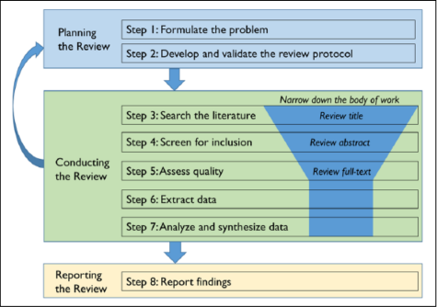
\includegraphics[width=0.5\linewidth]{figures/Review Phases.png}
    \caption{Detailed review phases}
    \label{fig:Review Phases}
 \end{center}
\end{figure*}


\subsection{Research questions and their motivations}

To respond to all the elements of our thesis many research questions were raised. The latter were also divided into sub-questions later on to find answers to more precise problems.

For this review, we will focus on the following 3 questions: 
\begin{enumerate}
    \item What is a recommender system and what are the different types and techniques used ?
    \item What is the knowledge used to define (i) the needs and profiles of users and (ii) business services ?
    \item How to use this knowledge to recommend a collection of business services while answering to the users requirements ?  (What are the current approaches that can benefit of such knowledge and can improve the autonomy (decrease frailty) of elderly)
\end{enumerate}

Table \ref{tab:RQ} displays the connection between the research questions and the research motivations.

\begin{table}
\centering
\footnotesize
\begin{tabularx}{\linewidth}{p{1cm}|X|X}
\toprule
&\multicolumn{1}{c|}{\normalsize\textbf{Research questions}} & \multicolumn{1}{c}{\normalsize\textbf{Motivations}} \\
\midrule
RQ1 &  What is a recommender system and what are the different types and techniques used ? & Understand what is a recommender system in general and in health care and identify the various techniques used.
             \\
RQ2 & What is the knowledge used to define (i) the needs and profiles of users and (ii) business services ? & Identify the knowledge necessary to generate a precise recommendation. Understand how users profile and needs are represented as well as the items recommended.
              \\
RQ3 & How to use this knowledge to recommend a collection of business services while answering to the users requirements and needs ? How can the recommender system improve the autonomy of elderly & Insure that users requirements and needs are met and the knowledge collected is well used.
             \\
RQ3' & What are the current approaches that can benefit of such knowledge and can improve the autonomy (decrease frailty) of elderly. & Finding out the current approaches employed to improve the autonomy (decrease frailty) of elderly and understand how they are applied.
            \\
\bottomrule
\end{tabularx}
\caption{Research questions and motivations}
\label{tab:RQ}
\end{table} 

\subsection{Research Strategies}

After finalizing the research questions, the research process took place. We used digital libraries since they give access to multiple contents with a potentially infinite number of resources and selections at hand. 

The list of libraries and databases used in this work is listed below: 
\begin{enumerate}
    \item Scopus (scopus.com)
    \item Web of Science (webofscience.com)
    \item Google Scholar (scholar.google.com)
\end{enumerate}



\begin{figure*}
 \begin{center}
    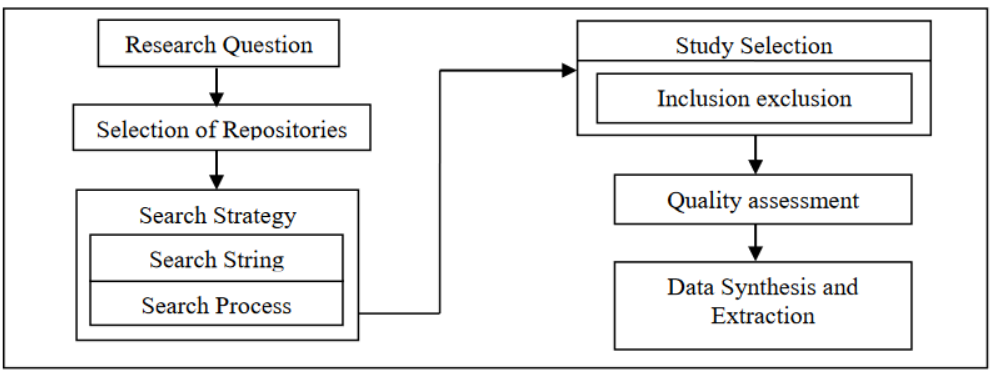
\includegraphics[width=0.5\linewidth]{figures/Review Protocol.png}
    \caption{Phase of review protocol}
    \label{fig:Review Protocol}
 \end{center}
\end{figure*}



Various search strings were used to get the final results. They were defined based on the research questions and the keywords of the research area.
Then they were improved by adding a list of synonyms as shown in Table \ref{tab:Keywords}

\begin{table}
\centering
\footnotesize
\begin{tabularx}{\linewidth}{p{3cm}|X}
\toprule
\multicolumn{1}{c|}{\normalsize\textbf{Keyword}} & \multicolumn{1}{c}{\normalsize\textbf{Synonym}} \\
\midrule
Recommender system &  Recommendation system, Recommending system, Advisor system
             \\
Frailty  & Fragility, Health, Healthcare, Health-Care, Well being, well-being, wellbeing, Autonomy, elderly
              \\
Service & Digital service, solution, activity, activities
             \\
User & User needs, User profile, Profiling, User model, Citizen
             \\
Model & Modeling, Knowledge modeling, MDE
            \\
Algorithmic &  Logic, programming
            \\
\bottomrule
\end{tabularx}
\caption{Research keywords and synonyms}
\label{tab:Keywords}
\end{table} 

\subsection{Study Selection}

To prevent any kind of bias or prejudice, internal validity and external validity supported the quality assessment in the selection process. That's how  
the identification of relevant papers was conducted in our work. 
We used Zotero as a reference management software in order to accumulate, store and organize the references. The inclusion and exclusion criteria of the papers are identified in the next section.


\subsection{Significant Journal Publications in Research}



\section{A Unified Framework for Risk and Business Processes Management}
\label{sec:bprim}
This paper develops a comprehensive, unifying and model-based framework named BPRIM for Business Process-Risk Integrated Method. It is a methodological framework based on the coupling of two typically separate parts - process management and risk management. This section describes the major components of the BPRIM framework: (1) The BPRIM life cycle (Section~\ref{sec:bprim:lifecycle}); (2) The BPRIM meta-model (Section~\ref{sec:bprim:metamodel}); and (3) The BPRIM modeling language (Section~\ref{sec:bprim:modelinglanguage}).

\subsection{BPRIM Life Cycle}
\label{sec:bprim:lifecycle} 
Applying BPM and ERM typically follows a procedural approach, known as the BPM life cycle and ERM life cycle, respectively. When aiming to integrate BPM and ERM, one naturally faces the challenge of integrating both life cycles. In the specific case of BPRIM, the challenge was to develop a life cycle that enables the design of risk-aware business process models. The BPRIM life cycle couples steps of the process management life cycle with those of risk management. This coupling can be made according to one of the following two approaches:
\begin{enumerate}
    \item A \emph{unification approach} that fuses different states of each individual life cycle to form a coherent whole. This approach requires the reconsideration of the logical activity sequences of each individual life cycle. The unified life cycle induces a significant change in the practices of BPM and ERM actors. It is a prescriptive approach, white box-like.
    \item An \emph{integration approach} is based on the principle of the black box and attempts to link the two individual life cycles by working on interfaces seeking to build relationships between their outputs and their respective inputs. This approach, which is descriptive, strengthens communication between the teams in charge of the cycles while minimizing changes to each individual life cycle. 
\end{enumerate}

In order to maintain the autonomy of business experts and risk experts and to facilitate the appropriation of BPRIM, we adopted the integration approach to design the BPRIM life cycle[X2,X4]. %~\cite{sienou_Bprim_integrating_06_X2,sienou_PhD_09_X4. 
The underlying assumption was that any activity is prone to risk and there is no risk without an associated activity. We therefore naturally chose the business process management life cycle as starting point. Consequently, the risk management life cycle will be driven by the process management life cycle. Indeed, in order to produce a new representation of the organization, i.e. the \textquote{To-Be} model, the description of how the organization works effectively, i.e. the \textquote{As-Is} model of the organization, must be defined before risks can be considered. Besides, it is the same vision that has been taken in the majority of the work on R-BPM \cite{jakoubi_roadmap_2010, conforti_supporting_2013, suriadi_current_2014}. This brings us to distinguish two major phases in the final cycle: a \emph{conceptual phase} associated with the design of the processes which are prone to risks; followed by an \emph{operational phase} concerned with the steering process led by risks.

In this work, the emphasis is on the conceptual phase of Risk-aware Business Process Management. In order to define the life cycle steps of this phase, we started from the BPM and the ERM life cycles that are most commonly accepted by their respective scientific communities, namely those proposed in \cite{dumas_fundamentals_2018,iso_iso_2009}. Then, we adopted a Structured Analysis for Real Time (S.A.R.T) method to study the information flows that can occur among the stages of the two cycles. This choice was motivated by the fact that we wanted to focus on the identification of existing interfaces between the different stages of the two isolated cycles and, in particular also, where data comes from, goes to, and where it will be stored. The S.A.R.T method is a structured analysis and design method which is widely used to graphically model these kind of data transformations in a system. It includes data-flow diagrams (DFD) to depict the data flow and supports decomposition mechanisms to display the inputs-outputs details of each component of the studied system \cite{von_scheel_phase_2015}.


\begin{figure*}[t]
 \begin{center}
    \includegraphics[width=0.8\linewidth]{figures/SARTLifeCycle3}
    \caption{Overview of interactions between process design stages and risk management stages}
    \label{fig:Overviewofinteractions}
 \end{center}
\end{figure*}

%TODO Please change the labels of the BPRIM models to be singular and capitalized like in Table 4, i.e., Business Process models -> Business Process Model
%done
%TODO Risk mapping -> Risk Mapping Model
%Done

Accordingly, we assumed that interaction will be primarily embedded in a set of models shared by the two cycles according to a supplier-consumer relationship. The result visualized in Figure~\ref{fig:Overviewofinteractions} is an alternating digraph which specifies all interactions between the two life cycles. The arcs are labelled to indicate the usage and storage of data in the target life cycle step or BPRIM model. Common models (items in bold in Figure~\ref{fig:Overviewofinteractions}) to steps of process design and risk management are placed in the centre of the graph. Generally, the BPRIM models act as database for the data to be created, used, and shared. The detailed description of these BPRIM models is given in Table~\ref{tab:BPRIMDiagrams}. An analysis of the graph in Figure~\ref{fig:Overviewofinteractions} leads to the following observations:
\begin{itemize}
    \item 
    The business process models are the main inputs for the \enquote{Setting the context} step of the ERM life cycle which aims to establish the scope of the risk management project. The steps of discovering business scenario, modeling processes, and setting the risk context are similar since they result in a set of models which support process and risk analysis.
    \item The steps of process analysis and risk analysis are related, which can be observed by the strong connectivity within these two stages in Figure~\ref{fig:Overviewofinteractions}. Indeed, the analysis step is based on the knowledge of risk analysis and risk assessment to guide the design of a new target process. In addition, the risk analysis is based on the results of the process analysis to determine risk levels, or propose criteria for classification of risks in a risk map.
\end{itemize}

\begin{figure*}[t]
 \begin{center}
    \includegraphics[width=0.99\linewidth]{figures/BPRIMLifecyclenew}
    \caption{BPRIM Life Cycle}
    \label{fig:BPRIMLifecycle}
 \end{center}
\end{figure*}

On the basis of these observations, we have completed this first flow-oriented modeling step in order to propose a coupling between the two life cycles which takes into consideration the temporal chronology. Indeed, the DFD-based modeling does not allow to study the temporal logic of the processes themselves. We chose Business Process Model and Notation (BPMN) to establish these models which are displayed in Figure ~\ref{fig:BPRIMLifecycle}. Following the temporal chronology of the comprehensive process and according to the similarity of the purposes sought by \enquote{Discover} and \enquote{Setting the context} activities, these latter shall be meld with \enquote{Model} activity into a scoping step that aims at setting up a context common to process design and risk management. The business model and the context model of risk are the main output of this common step.
By the same logic, \enquote{Analyze the processes} and \enquote{Analyze risks} activities shall be merged into a single activity. This latter should be incorporated then into a more comprehensive step which aims to assess process-related risks. 

The comprehensive analysis of the BPM and ERM life cycles models guided the design of the generalized Business Process Risk Integration Method (BPRIM) life cycle for Risk-aware Business Process Management at design-time (see Figure~\ref{fig:BPRIMLifecycle}). The iteractive BPRIM life cycle is triggered by a process-engineering environment and gradually enriched by a risk management process. It consists of the following four phases:
 \begin{enumerate}
     \item \textbf{Contextualize}: This phase aims at setting up the context of the joint management of risks and processes. It can be triggered by a decision affecting a significant change of the context such as the establishment of a new treatment alternative.
     \item \textbf{Assess}: This phase comprises the identification and implementation of the joint study of risks and processes to understand their interactions and possible impact. The outcome is necessary to prioritize risks and foster the development of risk treatment alternatives.
     \item \textbf{Treat}: This phase considers the definition of a set of treatment alternatives which triggers a new iteration of the assessment phase in order to understand the possible impact of the alternatives. This phase can lead to a reframing - meaning going back to the contextualization phase - which would require the implementation of risk handling actions. This is being done by fitting the models or by defining treatment alternatives. The risk handling scenarios that require no change of models will be stored to be triggered once needed.
     \item \textbf{Monitor}: In this phase, a monitoring takes place, checking whether decisions regarding treatment alternatives have been taken according to predefined instructions. It also ensures those alternatives which cannot be implemented through a simple change of process models at design-time will be transferred to be considered at deployment time. It is therefore a control phase, which provides guidance for refinement of the models or the transition to the implementation phase. However, at run-time phase, the handling of risks that evolves over time is carried out by a change in the model, which is compliant with the ISO 31000 specification. In other words, knowledge related to the model evolves with the real system behaviour (as depicted in Figure~\ref{fig:BPRIMLifecycle} by the cycle loop after the monitor activity). This is also the case for risks that have not been anticipated yet.
 \end{enumerate}
  
As we noted earlier, the information exchanged between these phases will be essentially contained in a wide range of BPRIM models and as displayed in Table ~\ref{tab:BPRIMDiagrams}. Based on model-driven engineering principles, these models must conform to a meta-model, which integrates concepts related to both, business processes and risks. The meta-model supporting the BPRIM method is developed in the next section.

\begin{figure*}[t]
    \centering
        \begin{subfigure}{0.66\textwidth}
         \begin{center}
            \includegraphics[width=0.99\linewidth]{figures/RiskMetaModel1}
            \caption{Excerpt of the Risk Meta-Model}
            \label{fig:RiskMetaModel}
         \end{center}
        \end{subfigure}
    \hfill
        \begin{subfigure}{0.33\textwidth}
         \begin{center}
            \includegraphics[width=0.99\linewidth]{figures/ValueConcept.png}
            \caption{The concept of value}
            \label{fig:ValueModel}
         \end{center}
        \end{subfigure}
    \caption{Risk Meta-Model excerpt (a) and specification of the concept of value (b)}
    \label{fig:relationsInMetamodel:Generic}
    \vspace{-.2cm}
\end{figure*}

\subsection{BPRIM Meta-Model}
\label{sec:bprim:metamodel}
The BPRIM meta-model specifies the main concepts handled during the different stages of the BPRIM life cycle and the allowed relationships between them. It considers the static aspects of BPRIM which guide and constrain the development of models. The BPRIM meta-model puts forward a conceptual unification of risks and processes into a common meta-model allowing to comprehensively address the semantics of R-BPM artefacts. The BPRIM meta-model was based on one hand on the business process meta-model proposed in the ISO 19440:2007 standard~\cite{iso_iso_2007} and on the other hand on our proposition of a risk meta-model [X2,X5]. %~\cite{sienou_Bprim_integrating_06_X2, sienou_Bprim_meta_model_08_X5}

The ISO 19440:2007 standard~\cite{iso_iso_2007} provides an abstraction level which fully matches conceptual modeling of business processes from the semantic point of view and offers guidelines which meet an organization’s needs. It consists of four parts, each linked to a point of view of the enterprise. The Organizational Management View describes the responsibilities and the authorities in the domain of the enterprise. The Information View describes the elements of information that represent the objects of the enterprise (material and informational objects) that are produced and used for the operations of the enterprise. The Resource View describes the assets and the resources of the enterprise (e.g., human resources, technology components). The Functions View describes the business processes, their functionality, behaviours, inputs, and outputs.



Concerning risk modeling, we have noted a lack of conceptual models playing a similar role as ISO 19440 for business processes modeling. This observation led to the proposition of a meta-model for risk, which is based on the study of the internal structure of risks. Figure~\ref{fig:RiskMetaModel} conceptualizes our vision of a risk meta-model. It defines risk with regard to the causal and the consequence perspectives. The causal aspect consists of risk factors that are favourable for the occurrence of a given risk event. Here, an event is an occurrence, which may cause state transitions within a system. This risk event is considered being the root cause of a risk situation, which describes a possible state of the system under study. The state is evaluated in terms of impact (positive or negative). The causality and the impact is interpreted by a set of actors while considering their interests, which is defined in the context of risk. Handling the risk to be acceptable is achieved by making decisions with regard to establishing control mechanisms affecting the cause or the consequence.

A subsequent mapping of relationships between these two meta-models is based on the concept of \emph{Value}. Undeniably, this concept of Value is a hotly debated issue in enterprise management (rules and values), in deployment of organizational strategy, in performance management, in design, in functional analysis, and in value-based management~\cite{philippe2003, bosch2007}. For example, we remind that business processes have been popularized as vectors of value creation by ~\cite[p.\ 38]{hammer1993}, who states that \emph{“a business process is a collection of activities that takes one or more kinds of inputs and creates outputs that is of value for the customer”}.

Considering most definitions, value creation seems to be a main characteristic of business processes. However, the concept of value seems to be ignored while conceptualizing business processes. In general, value designates the assessment of a value object by a given stakeholder. This assessment is either quantitatively or qualitatively evaluated in terms of value levels. A value describes the interest of a stakeholder for a given object and is interpreted by stakeholders. In this work, we follow the conceptualization of value as shown in Figure~\ref{fig:ValueModel}.

\newcommand\insertbprimsymbol[2][2cm]{%
  \raisebox{\dimexpr1.2em-\totalheight}{\includegraphics[width=#1]{figures/#2}}%
}
\newcommand\insertbprimrelation[2][.8em]{%
  \raisebox{\dimexpr#1-\totalheight}{\includegraphics[width=1.5cm]{figures/#2}}%
}

\begin{table*}[!ht]
	\centering
	\begin{tabularx}{\linewidth}{c|lX||clc|X}
	\toprule
        \multicolumn{3}{c||}{\textbf{BPRIM object types}}&
        \multicolumn{4}{c}{\textbf{BPRIM relation types}} \\
      
	 \midrule
      1 &\insertbprimsymbol{RiskFactor} & Characteristics of the system affecting the cause or the consequence of risk.
                 & 1 & \insertbprimrelation{InfluenceRelation} & 8 & \textbf{Influence} relation of a factor on an event. Inter-event influence relation. \\ 
                 \midrule
	   2 &\insertbprimsymbol{RiskSituation} & The state in which a risk event may lead the system. & 4 & \insertbprimrelation{ClassificationRelation} & 6
		         & Representation of the \textbf{belonging} of the risk to a
risk class. The direction indicates the class of risk.     \\ 
\midrule
		3 &\insertbprimsymbol{Value} & The value exposed to risk.& 4 &\insertbprimrelation{AggregationRelation} & 4
		         & Representation of the risk \textbf{aggregation} relationship.           \\ 
	\midrule
		4 &\insertbprimsymbol{Risk} & The possibility of a situation affecting an asset.& 4 &\insertbprimrelation{GeneralizationRelation} & 4
		         & Representation of the risk \textbf{generalization} relationship.  The direction indicates the general risk.           \\ 
		         \midrule
		5 &\insertbprimsymbol{Control} & Activities planed or executed in order to face a risk.& 8   & \insertbprimrelation{CausalityRelation} & 2
		         & \textbf{Causality} relation between an event and a risk situation.       \\ 
		         \midrule
	
		6 &\insertbprimsymbol{RiskClass} & Construct that represents a class including a breakdown structure of risks. & 2 & \insertbprimrelation{ImpactRelation} & 3
		         & \textbf{Impact} relation between risk situation and asset.       \\ 
		         \midrule
		7 &\insertbprimsymbol{RiskIndicator} & Construct that represents a risk indicator. & 4  &\insertbprimrelation[.4em]{GeneralAssociation} & 7
		         & \textbf{Association} which could outline relationship between risk and risk manager, or between risk and risk indicator.  \\ 
		            \midrule
		8 &\insertbprimsymbol{Event} & Construct that represents a non-risky related event. & 4 &\insertbprimrelation{RelationTarget} & *
		         &  \textbf{Affect} association which outlines that a given risk acts on a given business process concepts (process, activity, and object). \\ 
	    \midrule
		9 &\insertbprimsymbol{Stakeholder} & Organizational unit that is involved in risk assessment.& 3 & \insertbprimrelation{InterestRelation} & 9
		         & \textbf{Interest} relation between a stakeholder and an asset.             \\ 
	  \midrule
		10 &\insertbprimsymbol[0.65cm]{ANDOperator}\insertbprimsymbol[0.65cm]{OROperator}\insertbprimsymbol[0.65cm]{XOROperator} & AND operator, OR Operator and XOR Operator.& 4 &\insertbprimrelation{TreatmentRelation} & 5
		         & \textbf{Treatment} relation between risk and risk treatment measure.                                                                                \\ 
		         \bottomrule
	\end{tabularx}
\caption{Excerpt of the BPRIM modeling language for risk modeling}
\label{tab:BPRIMGraphicalNotation}
\end{table*}


Since a business process is a vector for value creation, a given object can be assessed different values by different stakeholders. For example, the performance is important for the process owner, while compliance is relevant to the quality manager and work safety to the risk manager. Furthermore, the consequence part of risk is evaluated in terms of impact. Since, risks are able to cause value modifications, it is easy to link a business process to a risk by defining the impact of the risk as a perception in the variation of the value level. Considering business processes, a risk is able to modify the value interpreted by a set of stakeholders. A risk may cause, for example, performance, quality or compliance variations. Risk-aware business process engineering is expected to provide means so that such variations could be controlled.

This understanding of the value concept allowed us to establish the relationships between the concepts provided by business process management and risk management. Figure~\ref{fig:BPRIMMetaModel} visualizes the core of the BPRIM meta-model for risk-aware business process management. Here, for instance, the business process is considered as being by itself a key value object of an organization. The values related to this object are expressed by key stakeholders of the organization. For clarification purpose, the process performance is for example a value. Any objects able to cause a performance variation is a risk factor that will increase the likelihood of occurrence of an instability (risk situation). Other meta-model elements contribute to semantically relate concepts of risk and process. Examples of such semantic relationships are the three different source/target relationships between risk, domain, business process, and enterprise activity, specifying the different kinds of elements responsible for either triggering a risk or being affected by a risk.

\subsection{BPRIM Modeling Language}
\label{sec:bprim:modelinglanguage}
The BPRIM language is designed to enable model-based risk-aware business process management. The starting point for the design of this language is the definition of the abstract syntax based on the integrated meta-model of Figure~\ref{fig:BPRIMMetaModel}. The second step is to define the concrete syntax, i.e., the graphical symbols used by the modeler to design and by the model user to easily interpret BPRIM models.

Given the intention to facilitate the appropriation of this new language, efforts have been made to reuse process modeling language concepts potential users are likely already familiar with. One of the most relevant languages that fits our needs is the Extended Event-Driven Process Chain (eEPC)~\cite{davis2007}. In a previously realized model mapping effort reported in [X4], % ~\cite{sienou2009},
we realized that eEPCs incorporate constructs and a graphical notation for modeling the majority of the concepts introduced by the ISO/DIS 19440 and support the view-based approach. Model views enable clear and precise representation of different aspects of an organization with different levels of abstraction. Another argument for choosing eEPC is its openness for extensions. For example, in an eEPC process diagram, one can graphically specify the objective of an activity and also the physical and human resources required for its implementation. It is important to note that this ability to represent the organizational elements with a sufficient level of detail (in terms of responsibility, role, and owner) is essential for risk analysis. Hence, it is worth highlighting that the BPMN language is not able to handle this crucial need since it neither permits to connect multiple resource allocations to the same activity, nor to model objectives. We point out that logical operators of EPC correspond to business rules in ISO/DIS 19440.

\begin{table}[h!]
	\centering
	\small
	\begin{tabularx}{\linewidth}{>{\raggedright}p{2.2cm}>{\raggedright}X>{\raggedright}p{2.2cm}>{\raggedright}X>{\raggedright}X}
\textbf{BPRIM model}  & \textbf{Aims} & \textbf{BPRIM\\Life cycle step} & \textbf{Content} & \textbf{BPRIM diagram} \tabularnewline 
\toprule
Business Process Model & Manage relationships and concepts specific to the company. & Contextualize & Business Process, Enterprise Activity, Event, Data Function, Information, Resource, Organizational unit, etc. &- Chain diagram for the macro process \newline 
- Organizational diagram \newline
- EPC diagram \tabularnewline 
\midrule 
Risk Context Model & Manages relationships among assets, stakeholders and values. & Contextualize & Organizational unit, Organizational role, Operational role, Value, etc. & - \textbf{\emph{Risk Context diagram}} \tabularnewline 
\midrule
Risk Analysis Model & Relates causes and consequences of risk. & Assess & Risk factor, Risk event, Risk situation, stakeholder, Value, etc. & - \textbf{\emph{Risk Analysis diagram}}\newline
- \textbf{\emph{Cause diagram}}\tabularnewline 
\midrule 
Risk Characterization Model & Characterize the risk in its environment & Assess & Risk, Risk class, Risk indicator, etc. & - \textbf{\emph{Risk extended EPC diagram}} \newline 
- \textbf{\emph{Risk diagram}} \newline
- \textbf{\emph{Risk Inventory diagram}} \newline 
- \textbf{\emph{Risk Relationship diagram}} \tabularnewline
\midrule
Risk Mapping Model  & Promote an overview of risk exposure and support action decisions. & Assess and Treat & Risk, Severity, Likelihood, Criticality. & - \textbf{\emph{Risk Mapping diagram}} \tabularnewline 
\midrule
Treatment Scenarios Model  & Manage treatment scenarios and understand their effects on risk mapping. & Treat & Control, Treatment, Risk, Risk Indicator, etc. & - \textbf{\emph{Risk extended EPC diagram}} \tabularnewline 
\bottomrule
\end{tabularx} 
\caption{Correspondences between BPRIM models and BPRIM diagrams in the process risk design cycle}
\label{tab:BPRIMDiagrams}
\end{table}

The BPRIM modeling language reuses eEPC constructs and notations and extends them with additional language constructs for risk-aware business process management by specialization (e.g. event, stakeholder, and process), new operators (e.g. operators between risk and treatment methods), and the related grammar with new relationships (e.g. compositional relationships, generalization between risks) [X2,X3,X6]. %~\cite{sienou_Bprim_language_07_X2, sienou_Bprim_language_08_X4, sienou_Bprim_language_09_X5}
Table~\ref{tab:BPRIMGraphicalNotation} lists the basic elements concerned with risk modeling in BPRIM with their graphical representation.

In order to simplify the inherent complexity of dealing simultaneously with risks and business processes, we have applied a viewing mechanism on top of the integrated BPRIM meta-model. This viewing mechanisms utilizes the complexity reduction mechanism of model viewing by concentrating on selected aspects individually. Consequently, the different views, represented as diagrams, use only a subset of the BPRIM modeling language which reduces the complexity of model creation for users and improves comprehension of models by human beings. The overarching BPRIM model is then re-constructed by combining the information covered in multiple views. Some of the BPRIM diagrams such as \emph{EPC} and \emph{Organigram} are well known in enterprise modeling and already integrated into several enterprise modeling tools. Others like the \emph{context diagram}, \emph{risk diagram}, and \emph{risk analysis diagram} have been newly introduced in order to meet the specific needs of BPRIM. Table~\ref{tab:BPRIMDiagrams} outlines the aims and content of the newly introduced BPRIM diagrams (using bold font).

\section{Implementation of \adobprim{} on ADOxx}
\label{sec:adobprim}
Technical feasibility of the BPRIM framework is evaluated by a conceptualization and implementation of BPRIM with the ADOxx meta-modeling platform~\cite{ADOxx}. This section briefly elaborates on the building blocks of ADOxx before the \adobprim{} tool will be presented.

\begin{table}[h]
	\centering
	\begin{tabular}{lcccccccccccc}
 \textbf{Framework} & \vtitre{Freeware License} & \vtitre{user-friendliness}&  \vtitre{Required knowledge}& \vtitre{Multi-user}  & \vtitre{Repository provision} & \vtitre{Supporting user-defined notations} & \vtitre{Supporting Multi-view modeling} & \vtitre{Supporting user-defined algorithms} & \vtitre{Object Configuration} & \vtitre{Querying objects } & \vtitre{Simulation} & \vtitre{Model checking and Validation}\\ 
 \toprule
 MetaEdit+ & No & \LEFTcircle & None & $\ocircle$ & \CIRCLE & \CIRCLE & \CIRCLE & \CIRCLE & \CIRCLE & $\ocircle$ & $\ocircle$ & \CIRCLE
\\ 
EMF (GEF, GMF) & Yes & $\ocircle$ & Java & $\ocircle$ & $\ocircle$ & \LEFTcircle & \CIRCLE & \CIRCLE & \CIRCLE & $\ocircle$ & $\ocircle$ & \CIRCLE
\\ 
Sirus & Yes & \LEFTcircle & Java & $\ocircle$ & $\ocircle$ & \LEFTcircle & \CIRCLE & \CIRCLE & \CIRCLE & $\ocircle$ & $\ocircle$ & \CIRCLE
\\ 
ADOxx & Yes & \CIRCLE & None & \CIRCLE  & \CIRCLE  & \CIRCLE & \CIRCLE & \CIRCLE & \CIRCLE & \CIRCLE  & \CIRCLE  & \CIRCLE
\\ 
MS DSL Tools & Yes & \LEFTcircle & C\# & $\ocircle$ & $\ocircle$ & \LEFTcircle & \CIRCLE & \CIRCLE & \CIRCLE & $\ocircle$ & $\ocircle$ & \CIRCLE
\\ 
Oryx & Yes & \CIRCLE & JSON & $\ocircle$ & $\ocircle$ & \CIRCLE & \CIRCLE & \CIRCLE & \CIRCLE & \CIRCLE & $\ocircle$ & \CIRCLE
\\

\midrule
\multicolumn{13}{l}{ $\ocircle$ \hspace{.1cm}=\hspace{.1cm} Not$ $ supported;  \quad \LEFTcircle \hspace{.1cm}=\hspace{.1cm} Partially $ $supported;  \quad \CIRCLE \hspace{.1cm}=\hspace{.1cm} Fully $ $ supported}\\
\bottomrule
\end{tabular}
\caption{Comparing several meta-modeling platforms}
\label{tab:MetaModelingEnv}
\end{table}

\subsection{ADOxx meta-modeling platform} 
To prepare the ground for the implementation of the BPRIM method as a modeling tool, we have investigated and analyzed several meta-modeling platforms such as (EMF)~\cite{mcneill2008}, Sirius~\cite{Sirius2014}, MetaEdit+~\cite{tolvanen2003}, Oryx~\cite{decker_oryx_2008}, MS DSL Tools~\cite{MSDSLTool} and ADOxx~\cite{ADOxx}. These paltforms usually provide many features required for the implementation of modeling tools for graphical modeling languages. The criteria used for the analysis of these platforms are derived from BPRIM requirements and presented in Table~\ref{tab:MetaModelingEnv}. The comparison focuses on the software licensing, the user-friendliness, the required knowledge, the collaborative functionality (e.g., multi-user, Repository provision), the ability to accommodate user-defined notations, to support multi-view modeling, to implement user-defined algorithms, to configure objects in models, to query models, to simulate models, and the ability to check models.

Compared to the others, ADOxx is a multi-user platform that provides a repository based on a relational database for meta-models and models. It is build upon the conceptual modeling framework visualized in Figure~\ref{fig:modelingmethodcomponents}. To introduce meta-models to ADOxx, no advanced knowledge of a programming language is required - in contrast to the use of the EMF with the Graphical Editing Framework (GEF) and the Graphical Modeling Framework (GMF) which requires a deep knowledge of the Java programming language. In addition, the ADOxx platform provides functionality which facilitates the management of models in the created modeling tool. For instance, ADOxx provides components and modules to analyze, simulate, and evaluate models. Besides, ADOxx has been widely used in industry and academia. In the past twenty years, tool support for more than 40 domain-specific modeling languages has been realized with ADOxx (see~\cite{OMiLAB-Book.2016} for an overview). Based on these observations, we have chosen the ADOxx platform to implement the BPRIM method and to realize the \adobprim{} tool.

\subsection{\adobprim{} Modeling Tool}
The main goal of the \adobprim{} modeling tool is to enable the graphical editing of artifacts conforming to the BPRIM meta-model. Moreover, \adobprim{} will enable to analyze, and asses risks of a business process by following the BPRIM life cycle. In this regard, we have adopted the approach advocated by~\citet{Bork.2010} to implement \adobprim{} with ADOxx. The approach is based on three stages:
\begin{enumerate}
    \item Introducing the modeling language by defining a mapping between the language concepts and the concepts provided by the ADOxx meta-metamodel~\cite{KaragiannisKuehn02};
    \item Designing the graphical visualization of the modeling language concepts in ADOxx;
    \item Implementing mechanisms \& algorithms which process the knowledge captured in the models, thereby increasing the value of the modeling method and the utility of the modeling tool and realizing the modeling procedure.
\end{enumerate}

\begin{figure}[t]
 \begin{center}
    \includegraphics[width=0.99\linewidth]{figures/AdoBPrimtool}
    \caption{Overview of the \adobprim{} modeling tool}
    \label{fig:MUP_BPRIM}
 \end{center}
\end{figure}
% "Risk analysis diagram" -> "Risk Analysis diagram"

Figure~\ref{fig:MUP_BPRIM} gives an overview of the realized \adobprim{} modeling tool. The \adobprim{} diagrams (see Table~\ref{tab:BPRIMDiagrams}) are realized as \emph{model types} in ADOxx and mapped to specific stages of the BPRIM life cycle (left side of Figure~\ref{fig:MUP_BPRIM}). By this structure, the \adobprim{} tool guides the user in choosing the right diagram according to the currently engaged BPRIM life cycle stage. As shown on the right side and bottom of Figure~\ref{fig:MUP_BPRIM}, the graphic notation palettes are contextualized according to the model type that the user has selected. In this regard, \adobprim{} supports multi-view modeling and hides complexity from the user. Based on the BPRIM life cycle, a modeling procedure has been realized which exploits the following mechanisms and algorithms:
\begin{itemize}
\item \textbf{Verification/Validation:} verification and validation functionalities are specified on different levels, ranging from \emph{cardinality checks} as syntactical checks (checking whether all constraints of the BPRIM modeling language are satisfied) to source-target validation. The objective of this mechanism is to ensure the accuracy of diagrams created by checking their structure according to several defined syntactic and semantic rules. 
\item \textbf{Risk Assessment:} The risk analysis model is analyzed and evaluated using a risk assessment matrix. The latter is a classical method to conduct qualitative risk assessment. The objective of this mechanism is to automatically produce a risk matrix which visualizes the different risk levels. To this end, some basic rules should be followed:
\begin{enumerate}
\item The basis for risks to happen is the standard definition of risk criticity as a combination of severity of the consequences and its likelihood. The output risk level is determined by the product of severity of consequences and likelihood, and illustrated in a two dimensional risk matrix.
\item Severity of consequences, likelihood, and risk level can be divided into different levels, respectively, with qualitative descriptions and scales. 
\item Definitions for the qualitative values (i.e. minor, major, medium, high, very high) were based on qualitative scales defined by the Haute Autorité de Santé (National Authority for Health in France- or HAS).
\item Based on the acceptance criteria, we defined three risk levels: low, moderate, and high.
\end{enumerate}
\end{itemize}

The tool has been developed as a project within the Open Models Laboratory, a worldwide community of modelers and modeling method developers~\cite{Bork:2019omilab}. A free download and further information on \adobprim{} are available through the corresponding project page\footnote{\adobprim{} project page [online]: \url{http://austria.omilab.org/psm/content/BPRIM/info}, last visited: 08.07.2019}.

\section{Experimentation and evaluation}
\label{sec:evaluation}
The aim of our experiment is: (1) to evaluate the capabilities of the BPRIM method to analyze risks and business processes in an integrated manner, (2) to determine its advantages and limitations compared to currently used methods, in particular the ALARM (Association of Litigation and Risk Management) method~\cite{vincent2000}, and (3) to identify potential improvements of the proposed approach. For reliable results, similarly to~\cite{barcelona2018}, we use a real world case study to evaluate our BPRIM framework. Indeed, we modeled and analyzed the medication-use process within an existing hospital in France.

This Section is structured as follows: Section~\ref{sec:experiment:context} briefly provides the context of the experimentation. The method used for conducting the experiment is then outlined in Section~\ref{sec:experiment:method}. Eventually, Section~\ref{sec:experiment:results} discusses the experimentation results with a focus on lessons learned and requirements for further improvements of BPRIM.

\subsection{Experiment Context}
\label{sec:experiment:context}

\begin{figure}[!ht]
 \begin{center}
    \includegraphics[width=0.99\linewidth]{figures/ADoBPRIM_excerpts_Models}
    \caption{Risk Context (top left), EPC (top right), Risk extended EPC (bottom left), and Risk Analysis (bottom right) diagrams in \adobprim{}}
    \label{fig:AdoBPRIM_use}
 \end{center}
\end{figure}
%TODO The name of the modeltypes are not capitalized as in Table 4.
% "Risk context diagram" -> "Risk Context diagram" etc..
%Done

The medication-use process is the fundamental system which provides the basis for safe medication use within the health care environment. Thus, ensuring medications are used and secured in the most appropriate manner and across all settings~\cite{Practice2019}. It consists in a complex and multidisciplinary process, involving numerous practitioners and it is composed of several stages (i.e. prescribing, dispensing, administration and medication monitoring). Indeed, it may involve up to 36 activities from the moment a doctor considers prescribing medication to the moment when this medication is actually administered or taken by the patient. 

This complexity causes a risk of Medication Errors (ME), which can involve serious consequences for the patients. Indeed, in 2015, the French National Authority for Health (FNAH) considers that 40\% of the serious adverse events are of medication error origin. For this reason, the safety of this process is at the heart of the guardianships in health care facilities. In 1995, the work of Leape and Bates~\cite{leape1995} radically changed the way people think about the causes of medication error. They highlighted that error is often the end result of a complex chain of events that either contributes to the error or renders it difficult to detect. Their work demonstrated the need for a systems approach to the medication error problem. Coupled with mounting public concern and awareness of the medication error problem, the physician and pharmacy leaders were sensitized to explore new approaches for medication error management~\cite{bevilacqua2018}.

Currently, some risk management methods are used in health care facilities. These methods essentially focus on teamwork (intervention of pharmacists, doctors, nurses and risk management team) to reduce the number of Adverse Drug Events (ADEs) due to medication errors. Specific structures, called Experience Feedback Committees (EFCs), were created to analyze ADEs within a medical department. An EFC is a multidisciplinary team representing the diversity of the functions encountered in the medical unit. The EFC members meet regularly to examine reported ADEs. The principle is to choose only one ADE per meeting in order to analyze it thoroughly and propose corrective actions. The choice is based either on the severity of the event or on its likelihood.

To analyze an ADE, the committee uses the so-called ALARM (Association of Litigation and Risk Management) method~\cite{vincent2000}. ALARM aims to get a picture-pause of the current situation and to identify the latent factors that have contributed to cause the ADE so as to set up error reduction strategies. Medication errors may be classified according to the stage of the medication-use process in which they occur (prescribing, dispensing, administration or monitoring).

The experiments have been conducted with the Intercommunal Hospital Center of Castres-Mazamet (CHIC) and focus on the quality control of its medication-use process for elderly in the Geriatric department. This choice is largely motivated by the fact that older adults are at a greater risk of medication errors. Indeed, they tend to take multiple medications (i,e, five or more prescribed drugs) during a day, referred as poly-pharmacy. In such multiple medication settings, quality and safety of the medication use process is highly sensitive.

\subsection{Experiment Method}
\label{sec:experiment:method}
The experiment was carried out in four main stages over a period of six months. Several actors of the CHIC were involved in this experiment, specifically two doctors, three nurses, two pharmacists, one pharmacy technician, and the Quality Manager of the hospital. 
\begin{itemize}
    \item In the first stage of experimentation, we observed the medication-use process in the Geriatric department at CHIC in order to define the study perimeter, to identify the involved stakeholders, and to create the as-is models of the medication-use process. At this stage, it’s worth noting that a training was provided for the identified stakeholders to introduce the main concepts of BPRIM and to show the use of the \adobprim{} tool. A focus at this stage was for participants to discover the different BPRIM diagrams and to understand their aims. The deliverable at this stage was one context diagram, four value-added chain diagrams and 14 EPC diagrams presenting a detailed functional and organizational view on the medication-use process in the Geriatric department. These diagrams were created and validated in collaboration with the experimentation team. All participants agreed on the models, representing the current way to perform the process.
    \item In the second stage we observed the risk management method which is currently used in this department. To this end, we have joined and participated in an Experience Feedback Committee meeting where an Adverse Drug Event was analyzed by a multidisciplinary team using the ALARM method.
    \item In the third stage of experimentation, we studied 10 real serious ADEs that have been reported by professionals related to the medication-use process in Geriatric department at CHIC. The ADEs had been analyzed by the EFC using the ALARM method. The aim of this stage was to analyze these ADEs with the BPRIM method and compare the gained results with those produced by the ALARM method. To this end, we analyzed, for each ADE, potential and reported facts and risk events that contribute to the ADE occurrence. Afterwards, we evaluated each ADE using the risk matrix defined by the French National Authority for Health (HAS). The deliverable at this stage was one BPRIM Risk diagram and one BPRIM Risk Analysis diagram for each ADE. After all ADEs were analyzed, a BPRIM Risk Map was produced that ranked all ADEs by criticality order (as shown in Figure~\ref{fig:AdoBPRIM_Matrix}). These diagrams were also subsequently validated by the experimentation team. This enabled us to trace advantages and current weakness of our approach.
    \item In the last stage of the experimentation we dealt with the validation and evaluation of the overall experiment results. It was performed in accordance with the stakeholders involved with this experimentation and other staff at CHIC. At this stage, value creation and preservation were deeply discussed.
\end{itemize}

The repository of models developed during the experimentation currently holds around 50 BPRIM models validated in collaboration with end-users (doctors and supporting project partners), some of which are presented in Figure~\ref{fig:AdoBPRIM_use}.

\begin{figure}[h!t]
 \begin{center}
    \includegraphics[width=0.99\linewidth]{figures/RiskMatrix}
    \caption{Evaluation of ADE accordingly to the French National Authority for Health recommendations}
    \label{fig:AdoBPRIM_Matrix}
 \end{center}
\end{figure}

\subsection{Experiment Results}
\label{sec:experiment:results}
This experimentation allows us to evaluate the feasibility and the relevance of the BPRIM framework with respect to its support of Risk-aware Business Process Management. Moreover, we are able to compare BPRIM to an existing method which was used at CHIC. Regarding the chosen application field, it is worth noting that people in charge of the medication-use process and health system at large, are not yet familiar with R-BPM approaches and that their risk management tools are often limited to the use of simple spreadsheet files listing the most frequent risks. This is why the use of the BPRIM framework has been proved more efficient than the traditional method since it was able to formalize more knowledge about risks allowing more comprehensive analysis in a business process context. BPRIM evolves the state of the art from survey based methods with literal means of investigation and analysis to a graphic based method with algorithms.

By carrying out a critical view of the used risk method in CHIC, we can say that error is often the end result of a complex chain of various factors and risk events that contributes to the ADEs occurrence. Therefore, analysis of ADEs should focus on the vulnerabilities of the medication-use process rather than on individual errors. Thus, key to analyzing ADEs is a well understood medication-use process that sheds light to the vulnerabilities and weaknesses related to the organization. This is why the BPRIM method recommends to create an as-is view of the system under study prior to the analysis stage.

Thanks to the \adobprim{} tool, we efficiently designed more than 50 diagrams that allowed us to place the identified risks in their business process context and to automatically evaluate them in order to prioritize the potential risks. As a result, a broader knowledge base has been established, which is useful for the effective management of the hospital medication-use process and compliance control. This knowledge base was shared, thanks to \adobprim{}, among several actors involved within this process for checking and validation.

This experimentation revealed that new users of \adobprim{} easily adopted the tool which enabled them to enhance the knowledge base by adding several new diagrams and linking them to other related diagrams. Users also argue on the gain they will achieve by sharing the knowledge base with colleagues. Indeed, it allows them to have a comprehensive vision of risks which is not limited to the medical department which they belong to, as it was the case with the ALARM method. It has been also valued as a useful brainstorming tool for improving the quality of pharmacological management as well as the patient care processes.

Besides, undertaking this experimentation has led to figure out three major weaknesses of the current prototype of the \adobprim{} tool which will be dealt with in future versions. The first one is related to consistency of multi-view models. As shown in Figure~\ref{fig:BPRIMMetaModel}, BPRIM Meta-model comprises views on risk, business process, organization, and value. These multiple views bring inevitable syntactically and semantically overlaps  when establishing the different diagrams under \adobprim{}. In this context, it will be crucial for the utility and the applicability of our multi-view modelling method to keep these multiple views consistent and provide suitable visualizations. The second weaknesses concerns the risk evaluation method implemented in \adobprim{}. Currently, we only use a qualitative method. It will be also interesting to integrate quantitative evaluation methods for a more comprehensive risk analysis. The third weakness points out to the lack of algorithms and mechanisms in order to study the risks propagation and their impact on values created by activities and which are interesting for stakeholders.

\section{Conclusion}
\label{sec:conclusion}
Risk consideration in enterprise engineering is of increasing importance since the business environment is becoming more and more competitive and unpredictable. This need has given rise to the risk-aware business process management (R-BPM) paradigm. It consists of the integration of risk aspects into business process management in order to increase the risk-awareness of an organization's business processes. R-BPM aims to improve global performance and robustness of business process management by enabling a strong collaboration between process and risk management teams.

Investigations and literature analysis that we conducted revealed the weakness of this paradigm with regard to maturity and theoretical foundations, which is necessary for structure, experiments and comprehensiveness, for the scientists as well as for professional practitioners. This research was therefore motivated by these needs.

Our main contribution consists in the design of the BPRIM framework as a path toward the first foundations for risk-aware business process management. Adopting the vision of method concept from information technologies and drawing upon the principles of enterprise architecture, BPRIM suggests an integrative approach with three components:
\begin{itemize}
    \item A BPRIM life cycle based on coupling the stages of existing BPM and ERM life cycles. Considering information exchanged between the synchronized life cycle of process design and risk management, a set of models was identified and realized as diagrams regarding the input and output of each step.
    \item A conceptual unification of risk and process based on the coupling between the process meta-model proposed by the ISO/DIS 19440 and the risk meta-model that we have defined at a generic level. In this context, the concept of value has played the role of keystone between these two meta-models. 
    \item A semi-formal graphical modeling language with meta-model and notation. We extended the ISO/DIS 19440 constructs with a new set of constructs for risk modeling. The outcome is a model, which is considered as the abstract syntax of risk enriched process-modeling languages. In order to support an operational usage, a visual concrete syntax is proposed by extending the eEPC notation.
\end{itemize}

For modeling artefacts conforming to the BPRIM language and automatically assessign risks at a business process level following to the BPRIM life cycle, a dedicated modeling tool called \adobprim{} has been built on the ADOxx platform and was may openly available through the OMiLAB~\cite{Bork:2019omilab}.

For evaluation purposes we applied the BPRIM method and the \adobprim{} tool to the quality control of pharmacological management in a French hospital. We have chosen this application domain because the medication-use process in hospitals is a complex and knowledge-intensive one. Here, any process stage is indeed a source of potential errors that may cause risks to the patient’s health. It is also a highly regulated process for which risk management practices have become an imperative by public authorities. 

Thanks to the BPRIM method, we have analyzed risks in their business process context and we were able to evaluate them accordingly. The results obtained thanks to the \adobprim{} tool were verified and validated by professionals in the field and were largely concordant or even more relevant in several cases than those obtained by the currently used method. Of course, this method is not limited to the health care sector. The generic character of the BPRIM meta-model makes it usable to any other sector, such as civil engineering, transportation, crisis management, etc.

Besides, the feedback gained from the experiment reveals few shortcomings about the current version of the \adobprim{} implementation which remain acceptable given its young maturity which is emphasized on the design-time stage. To overcome these weaknesses, we are currently working on a new version of \adobprim{}, which will integrate new functionalities for risk management. We intend to enhance the run-time stage by adding new features to the modeling environment such as simulation capabilities to: study risk propagation, evaluate risk impact, and stress test control mechanisms. To these ends, currently the laboratory is conducting PhD research on business continuity management and risk propagation analysis methods, the results of which will refine the proposed BPRIM method and extend the \adobprim{} tool.

\section*{Acknowledgement}
The authors would like to show their gratitude to the Intercommunal Hospital Center of Castres-Mazamet and more specifically Dr. CUFI, the head of the Geriatric Department and Dr. CLEOSTRATE, the head of Inpatient Pharmacies who allowed us to evaluate our BPRIM method and \adobprim{} tool on a real case and provided insights and expertise that greatly enhanced this research. We would also like to thank OMiLAB members for assistance with the ADOxx platform and for providing a collaborative space on their OMiLAB portal.

\section*{References}

\bibliographystyle{model1-num-names}
\bibliography{sample.bib}

%% Authors are advised to submit their bibtex database files. They are
%% requested to list a bibtex style file in the manuscript if they do
%% not want to use model1-num-names.bst.

%% References without bibTeX database:

% \begin{thebibliography}{00}

%% \bibitem must have the following form:
%%   \bibitem{key}...
%%

% \bibitem{}

% \end{thebibliography}

\end{document}
